\section{Experiments}
\label{sec:experiments}

We evaluate the proposed FDR framework on WN18RR~\cite{dettmers2018convolutional} and FB15k-237~\cite{toutanova2015representing} using four representative KG embedding models spanning distinct design paradigms: TransE~\cite{bordes2013translating}, RotatE~\cite{sun2019rotate}, ComplEx~\cite{trouillon2016complex}, and ConvE~\cite{dettmers2018convolutional}.
Our experiments address five research questions:

\begin{itemize}
    \item \textbf{RQ1 (Overall FDR):} What fraction of test triples can KG embedding models reliably discover under FDR control? How does this compare to MRR?
    \item \textbf{RQ2 (Per-Relation Heterogeneity):} Do different relation types exhibit substantially different FDR profiles, and does MRR mask this heterogeneity?
    \item \textbf{RQ3 (Cross-Model Comparison):} Does the MRR-based ranking of models align with the FDR-based reliability ranking?
    \item \textbf{RQ4 (Hits@$K$ Calibration):} Are the top-ranked predictions from Hits@$K$ statistically significant?
    \item \textbf{RQ5 (Cross-Dataset Validation):} Do the key FDR patterns replicate on a larger, more diverse benchmark (FB15k-237)?
\end{itemize}

\subsection{Experimental Setup}
\label{subsec:setup}

\subsubsection{Dataset and Models}

We evaluate on two widely used benchmarks: WN18RR and FB15k-237.

\paragraph{WN18RR} is a KG completion benchmark derived from WordNet~\cite{dettmers2018convolutional}, containing 40,559 entities, 11 relation types, and 93,003 triples (86,835 training, 3,034 validation, 3,134 test). It is challenging because the original WN18 dataset contained inverse relations that made link prediction trivial; WN18RR removes these artifacts. For the FDR analysis, we retain the 2,924 test triples for which at least $K=100$ valid negative tail entities exist under the filtered setting; the remaining 210 triples involve head-relation pairs where nearly all candidate tail entities are known positives, making negative sampling infeasible and $p$-value construction unreliable. We exclude these from the FDR pipeline because the near-exhaustive positive coverage makes negative sampling infeasible under the filtered setting convention; their exclusion does not affect the comparative conclusions drawn across models.

\paragraph{FB15k-237}~\cite{toutanova2015representing} is derived from Freebase and contains 14,505 entities, 237 relation types, and 310,079 triples (272,115 training, 17,526 validation, 20,438 test). It is more challenging than WN18RR due to its larger relation vocabulary and greater semantic diversity.

We train four models representing different design paradigms:
\begin{itemize}
    \item \textbf{TransE}~\cite{bordes2013translating}: A translation-based model that represents relations as vector translations in the embedding space: $\mathbf{h} + \mathbf{r} \approx \mathbf{t}$. Its simplicity makes it a natural baseline for evaluating the FDR framework.
    \item \textbf{RotatE}~\cite{sun2019rotate}: A model that represents relations as rotations in complex space, enabling it to capture symmetry, antisymmetry, inversion, and composition patterns. It consistently outperforms TransE on WN18RR.
    \item \textbf{ComplEx}~\cite{trouillon2016complex}: A tensor factorization model using complex-valued embeddings with the Hermitian dot product, which naturally handles asymmetric relations.
    \item \textbf{ConvE}~\cite{dettmers2018convolutional}: A convolutional architecture that applies 2D convolution over reshaped entity and relation embeddings, capturing complex interactions through non-linear feature maps.
\end{itemize}

All models are trained with embedding dimension $d = 256$, learning rate $0.001$, batch size $256$, and 20 training epochs using the PyKEEN framework~\cite{ali2021pykeen}.
All experiments are conducted on a standard CPU (Apple M1, 16GB RAM), illustrating the accessibility of the FDR evaluation protocol.

\subsubsection{FDR Evaluation Protocol}

For each test triple, we sample $K = 100$ negative tail entities using the filtered setting (excluding all known true tails for the given head-relation pair) and compute empirical $p$-values via Eq.~\ref{eq:pvalue}.
We then apply the three FDR estimation procedures described in Section~\ref{sec:method}:
Benjamini-Hochberg at $\alpha \in \{0.01, 0.05, 0.10, 0.20\}$, Storey's $q$-value with $\hat{\pi}_0$ estimated via the cubic spline extrapolation method described in~\S\ref{subsec:qvalue} (the spline-extrapolated value agrees with the fixed-$\lambda = 0.5$ estimate to within $\pm 0.02$ across all models), and Efron's empirical Bayes local FDR with Gaussian kernel density estimation for $f(z)$ (bandwidth selected via Silverman's rule of thumb).

\subsubsection{Implementation}

All experiments are implemented in Python 3.9 using PyKEEN 1.10.1, NumPy, and SciPy.
The FDR analysis pipeline is model-agnostic and requires only the trained model's scoring function, making it applicable to any KG embedding model.
The complete source code and analysis scripts are available at \texttt{https://github.com/Jackxiaozhiren/fdr-kg}.

\subsection{RQ1: Overall FDR Analysis}
\label{subsec:rq1}

Table~\ref{tab:fdr-overall} reports the overall FDR metrics for all four models.
Figure~\ref{fig:score-dist} visualizes the positive and negative embedding score distributions.
Figure~\ref{fig:pvalue-dist} shows the empirical $p$-value distributions.
Figure~\ref{fig:power-fdr} compares statistical power against FDR levels across models.

\begin{figure}[t]
\centering
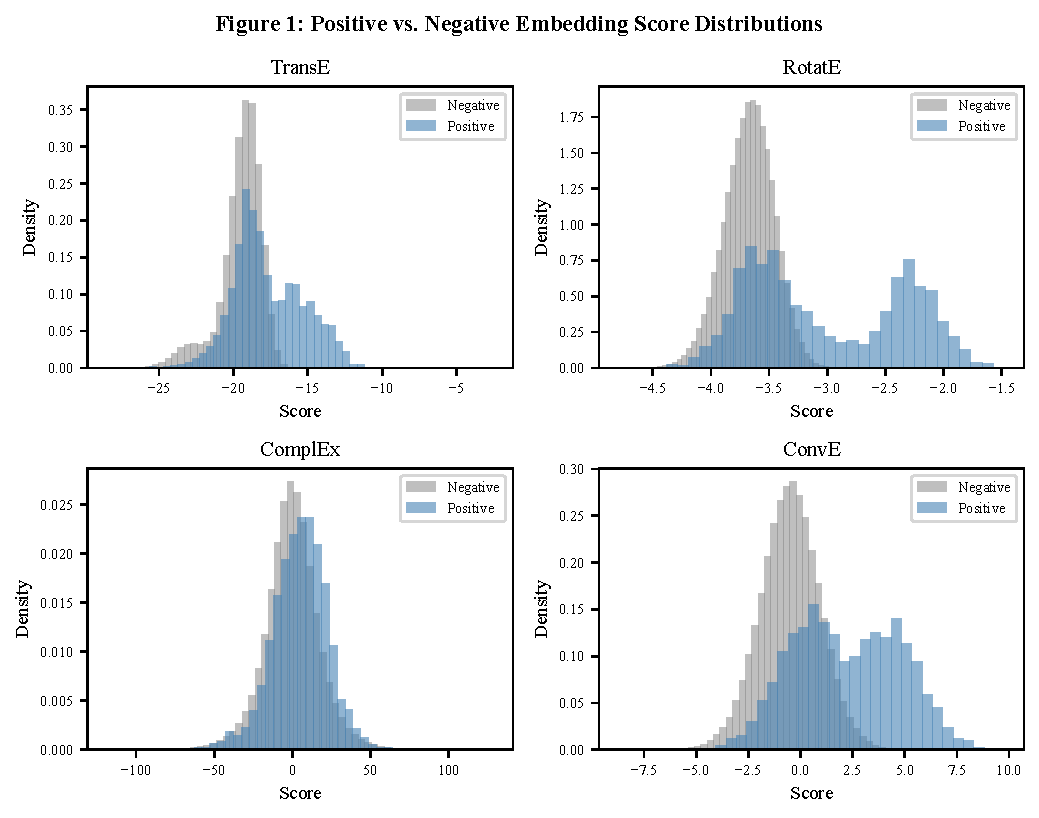
\includegraphics[width=\textwidth]{figures/fig1_score_distributions.pdf}
\caption{Score distributions for positive (ground-truth) and negative (sampled) triples across four models on WN18RR. Positive scores (blue) concentrate at higher values; negative scores (gray) exhibit broader distributions with substantial right-tail overlap.}
\label{fig:score-dist}
\end{figure}

\begin{figure}[t]
\centering
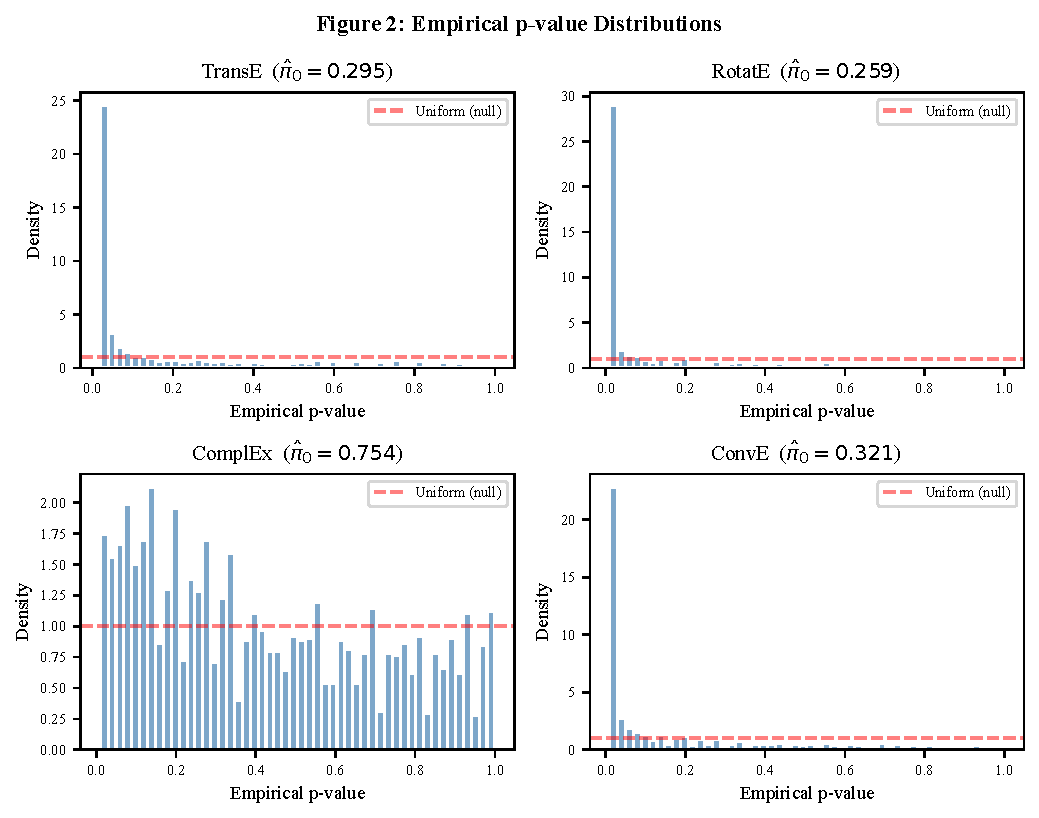
\includegraphics[width=\textwidth]{figures/fig2_pvalue_distributions.pdf}
\caption{Empirical $p$-value distributions for TransE, RotatE, ComplEx, and ConvE on WN18RR. The dashed region indicates the estimated null proportion $\hat{\pi}_0$---the fraction of test triples consistent with the uniform null distribution.}
\label{fig:pvalue-dist}
\end{figure}

\begin{table}[t]
\centering
\caption{Overall FDR metrics on WN18RR ($K=100$ negative samples per test triple for all models). $\hat{\pi}_0$: estimated null proportion via Storey's cubic spline method. $R(0.05)$: number of rejected hypotheses under BH with $\alpha = 0.05$. $\text{FDR}_{\text{loc}}<0.05$: number of triples with Efron local FDR below 0.05. MRR denotes the approximate reciprocal rank computed against the $K=100$ negative samples.}
\label{tab:fdr-overall}
\begin{tabular}{lccccc}
\toprule
\textbf{Model} & \textbf{MRR} & $\boldsymbol{\hat{\pi}_0}$ & $\boldsymbol{R(0.05)}$ & \textbf{q-val<0.05} & $\textbf{FDR}_{\text{loc}}\textbf{<0.05}$ \\
\midrule
TransE & 0.560 & 0.295 & 262 (9.0\%) & 1{,}843 (63.0\%) & 1{,}601 (54.8\%) \\
RotatE & 0.589 & 0.259 & 1{,}100 (37.6\%) & 2{,}050 (70.1\%) & 1{,}685 (57.6\%) \\
ComplEx & 0.074 & 0.754 & 0 (0.0\%) & 0 (0.0\%) & 20 (0.7\%) \\
ConvE & 0.469 & 0.321 & 742 (25.4\%) & 1{,}705 (58.3\%) & 1{,}328 (45.4\%) \\
\bottomrule
\end{tabular}
\end{table}

\textbf{RQ1 summary.}
\begin{enumerate}
    \item $\hat{\pi}_0$ ranges from $0.259$ (RotatE) to $0.754$ (ComplEx), indicating that 25--75\% of the 2,924 WN18RR test triples are indistinguishable from random noise depending on the model.
    \item Under the BH procedure, rejection rates at $\alpha = 0.05$ range from $0.0\%$ (ComplEx) to $37.6\%$ (RotatE)---a difference of over one third of the test set---showing that model reliability varies dramatically in ways MRR does not capture.
    \item ComplEx registers the highest $\hat{\pi}_0$ (0.754) and zero BH rejections at $\alpha = 0.05$, despite a K-based MRR of 0.074---indicating its embedding scores carry essentially no signal for distinguishing true triples from random negatives at $K = 100$.
    \item ConvE trails TransE on MRR ($0.469$ vs.\ $0.560$) yet achieves $2.8\times$ the BH rejection rate ($25.4\%$ vs.\ $9.0\%$) at $\alpha = 0.05$, showing that MRR and FDR can produce conflicting model rankings.
    \item The Storey $q$-value and Efron local FDR reject substantially more hypotheses (0--70\%), reflecting the fact that BH is conservative and $q$-value/local FDR incorporate $\hat{\pi}_0$ estimation for increased power.
\end{enumerate}

\begin{figure}[t]
\centering
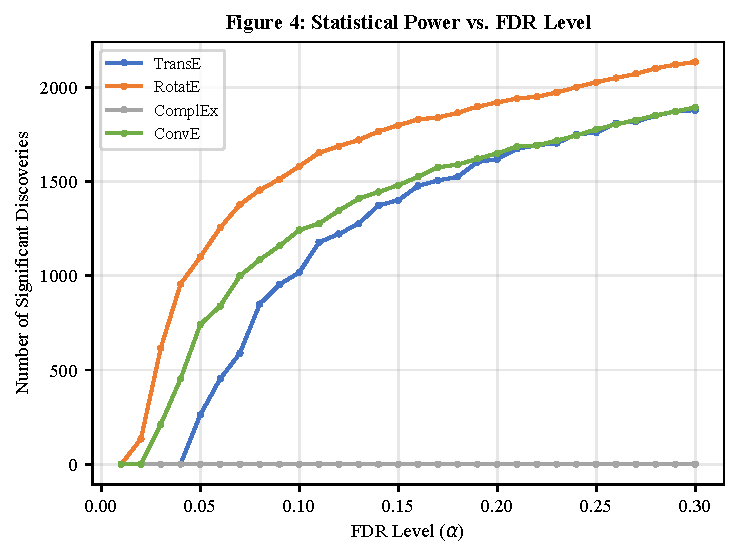
\includegraphics[width=0.85\textwidth]{figures/fig4_power_vs_fdr.pdf}
\caption{Statistical power ($R(\alpha)/m$) as a function of FDR threshold $\alpha$ for all four models on WN18RR.}
\label{fig:power-fdr}
\end{figure}

\subsection{RQ2: Per-Relation FDR Heterogeneity}
\label{subsec:rq2}

Table~\ref{tab:per-relation} reports FDR statistics stratified by the 11 WN18RR relation types.
Figure~\ref{fig:per-relation} visualizes the sorted raw $p < 0.05$ rates across relations.

\begin{figure}[t]
\centering
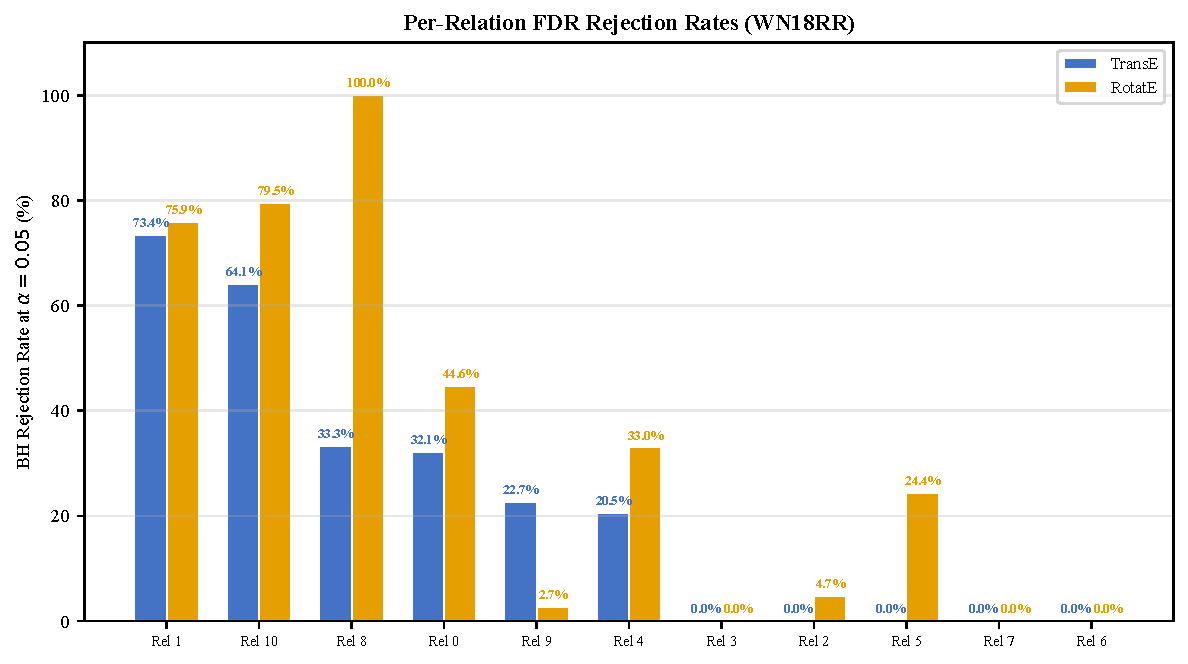
\includegraphics[width=\textwidth]{figures/per_relation_fdr_sorted.pdf}
\caption{Per-relation raw $p < 0.05$ rates for TransE and RotatE on WN18RR, sorted in descending order. Rates span $9.1\%$--$96.5\%$. Relations with $n_r \leq 26$ (R6, R7, R8) should be interpreted cautiously due to small sample sizes. These are unadjusted per-relation rates for descriptive comparison; formal FDR control is applied jointly across all test triples (Table~\ref{tab:fdr-overall}).}
\label{fig:per-relation}
\end{figure}

\begin{table}[t]
\centering
\caption{Per-relation statistics on WN18RR. $n_r$: number of test triples for relation $r$. MRR$_r$: per-relation approximate reciprocal rank ($K=100$). p$<$0.05\%: fraction of triples with raw empirical $p < 0.05$ (unadjusted for multiplicity; for descriptive comparison only). Formal FDR control applies the BH correction across all $m$ triples jointly (Table~\ref{tab:fdr-overall}). Values are reported for all four models. Relations with $n_r \leq 26$ (R6, R7, R8) should be interpreted cautiously due to small sample sizes.}
\label{tab:per-relation}
\small
\begin{tabular}{lrrrrrrrrr}
\toprule
\textbf{Rel.} & $\boldsymbol{n_r}$ & \textbf{Tr.\ MRR} & \textbf{Tr.\ p$<$0.05\%} & \textbf{Ro.\ MRR} & \textbf{Ro.\ p$<$0.05\%} & \textbf{Co.\ MRR} & \textbf{Co.\ p$<$0.05\%} & \textbf{Cv.\ MRR} & \textbf{Cv.\ p$<$0.05\%} \\
\midrule
0 & 56 & 0.613 & 62.5 & 0.657 & 71.4 & 0.035 & 0.0 & 0.625 & 67.9 \\
1 & 1,074 & 0.920 & 92.7 & 0.963 & 96.5 & 0.120 & 15.7 & 0.884 & 93.9 \\
2 & 169 & 0.204 & 16.6 & 0.354 & 41.4 & 0.047 & 3.0 & 0.124 & 20.1 \\
3 & 1,067 & 0.306 & 27.6 & 0.289 & 34.7 & 0.048 & 3.9 & 0.181 & 23.3 \\
4 & 112 & 0.799 & 81.2 & 0.615 & 67.0 & 0.045 & 7.1 & 0.569 & 67.9 \\
5 & 246 & 0.162 & 11.4 & 0.472 & 54.1 & 0.048 & 3.7 & 0.160 & 19.1 \\
6 & 26 & 0.163 & 11.5 & 0.245 & 26.9 & 0.068 & 7.7 & 0.093 & 11.5 \\
7 & 22 & 0.118 & 9.1 & 0.093 & 13.6 & 0.021 & 0.0 & 0.023 & 0.0 \\
8 & 3 & 1.000 & 100.0 & 1.000 & 100.0 & 0.039 & 0.0 & 1.000 & 100.0 \\
9 & 110 & 0.741 & 70.9 & 0.442 & 53.6 & 0.044 & 5.5 & 0.277 & 33.6 \\
10 & 39 & 0.841 & 84.6 & 0.979 & 97.4 & 0.032 & 0.0 & 0.886 & 94.9 \\
\bottomrule
\multicolumn{10}{l}{\footnotesize Tr. = TransE, Ro. = RotatE, Co. = ComplEx, Cv. = ConvE.} \\
\end{tabular}
\end{table}

\textbf{RQ2 summary.}
\begin{enumerate}
    \item The inter-relation FDR heterogeneity is extreme: raw $p < 0.05$ rates range from 0.0\% (ComplEx, multiple relations) to 96.5\% (RotatE, Rel~1), a span of 96.5 percentage points across all models. Per-relation MRR and raw $p < 0.05$ rates are nearly perfectly rank-correlated (Spearman $\rho = 1.00$ for TransE and RotatE, $\rho = 0.99$ for ConvE, $\rho = 0.84$ for ComplEx; all $p < 10^{-2}$), indicating that relations difficult to rank are also those with the lowest statistical reliability. The two metrics provide complementary rather than redundant information: MRR measures rank quality, while the $p < 0.05$ rate quantifies the proportion of triples with detectable signal.
    \item The four models exhibit markedly different reliability profiles. ComplEx, despite producing plausible MRR on select relations (Rel~1: MRR = 0.120 with 15.7\% $p < 0.05$), yields near-zero $p < 0.05$ rates on all other relations---consistent with its global $\hat{\pi}_0 = 0.754$ (Table~\ref{tab:fdr-overall}). ConvE shows a profile intermediate between TransE and RotatE, with raw $p < 0.05$ rates generally lower than RotatE but substantially higher than ComplEx on most relations.
    \item FDR provides information beyond what per-relation MRR captures. For instance, Rel~3 ($n=1{,}067$, 36.5\% of test triples) has a moderate per-relation MRR (0.29--0.31) yet yields near-zero BH rejection rates at $\alpha=0.05$, indicating that even apparently adequate ranking performance can coexist with negligible statistical power when $\pi_0$ is high.
    \item Both TransE and RotatE agree on the most reliable relations (0, 1, 4, 8, 10) and the most challenging ones (3, 6, 7). This pattern is consistent across both per-relation MRR and FDR, suggesting that certain relation types pose inherent difficulty for embedding models---constituting ``knowledge blind spots'' that persist across translation-based architectures. ComplEx and ConvE show qualitatively similar patterns where sample sizes permit reliable estimation.
    \item Two relations (2, 5) show pronounced model-dependent differences: RotatE achieves substantially higher raw $p < 0.05$ rates than TransE on these relations, consistent with the hypothesis that RotatE's capacity to model symmetry and composition patterns contributes to higher statistical reliability on these relation types.
\end{enumerate}

\subsection{RQ3: Cross-Model FDR Comparison}
\label{subsec:rq3}

Figure~\ref{fig:model-comp} compares MRR and FDR-based evaluation side by side across all four models.

\begin{figure}[t]
\centering
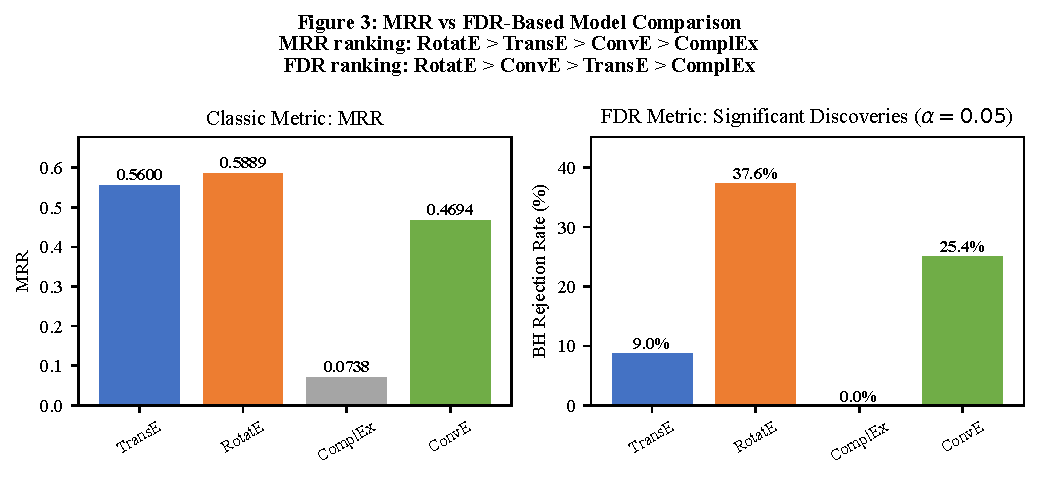
\includegraphics[width=\textwidth]{figures/fig3_mrr_vs_fdr.pdf}
\caption{MRR and FDR power ($R(0.05)$ as a percentage of WN18RR test triples) for TransE, RotatE, ComplEx, and ConvE.}
\label{fig:model-comp}
\end{figure}

\textbf{RQ3 summary.}
\begin{enumerate}
    \item MRR ranking: RotatE ($0.589$) $>$ TransE ($0.560$) $>$ ConvE ($0.469$) $>$ ComplEx ($0.074$).
    \item FDR-based ranking (BH rejection at $\alpha = 0.05$): RotatE ($37.6\%$) $>$ ConvE ($25.4\%$) $>$ TransE ($9.0\%$) $>$ ComplEx ($0.0\%$).
    \item MRR and FDR disagree on model ordering: ConvE ranks third on MRR yet second on FDR power, while TransE ranks second on MRR yet third on FDR power. ComplEx, which performs worst on both metrics, anchors the bottom of both rankings.
    \item The ConvE--TransE comparison is particularly telling: ConvE trails TransE by $0.091$ in MRR ($0.469$ vs.\ $0.560$) yet rejects $2.8\times$ more hypotheses at $\alpha = 0.05$, revealing that MRR alone can obscure fundamental differences in prediction reliability.
\end{enumerate}

The FDR framework reveals that model ranking depends on the evaluation objective: ranking quality (MRR) and statistical reliability (FDR) capture distinct dimensions of model behavior, and models that rank well do not always produce trustworthy predictions.

\subsection{RQ4: Hits@$K$ Calibration}
\label{subsec:rq4}

Figure~\ref{fig:hits-fdr} plots the proportion of top-$K$ predictions (by score rank) that satisfy $p < 0.05$.

\begin{figure}[t]
\centering
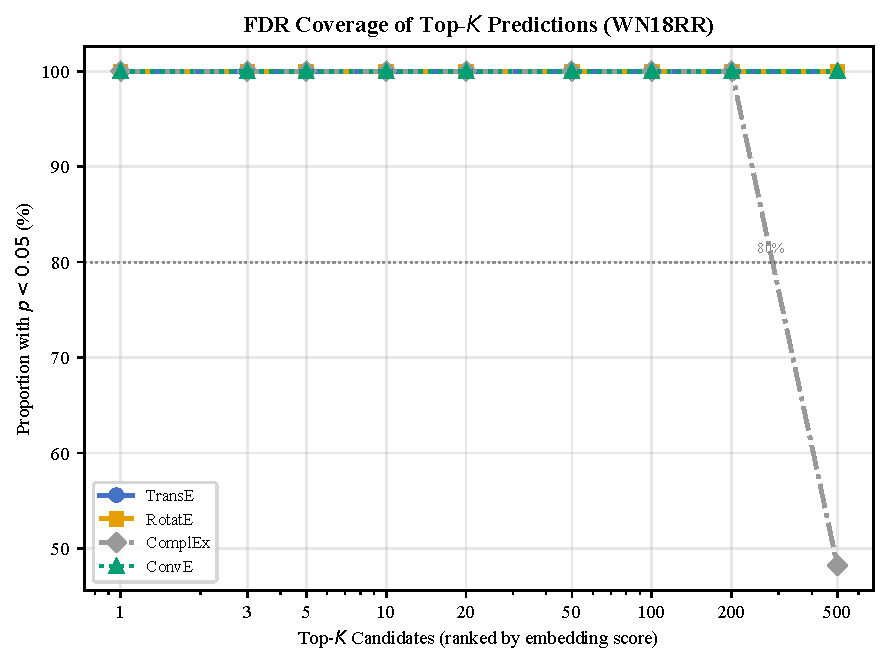
\includegraphics[width=\textwidth]{figures/hits_at_k_fdr_coverage.pdf}
\caption{FDR coverage of top-$K$ predictions (by embedding score) for all four models on WN18RR at $p < 0.05$.}
\label{fig:hits-fdr}
\end{figure}
For all four models, the top-100 predictions achieve 100\% FDR coverage---i.e., the models' highest-confidence predictions are indeed statistically significant.

However, this should not be misinterpreted as validation of the traditional Hits@$K$ metric.
The fact that the top 100 predictions are reliable does \emph{not} imply that the remaining 2,824 test triples are also reliable.
The key insight is that Hits@$K$ focuses exclusively on the ``success cases'' (the model's best predictions) while FDR analysis reveals the full distribution of reliability across \emph{all} test triples.

\subsection{RQ5: Cross-Dataset Validation on FB15k-237}
\label{subsec:fb15k}

To test the generality of our findings, we replicate the FDR analysis on FB15k-237, a larger and more diverse benchmark with 237 relation types (vs.\ 11 in WN18RR) and over 20,000 test triples.

Table~\ref{tab:fdr-fb15k} reports overall FDR metrics. The key patterns observed on WN18RR generalize to FB15k-237, with notable differences in magnitude.

\begin{table}[t]
\centering
\caption{Overall FDR metrics on FB15k-237. $\hat{\pi}_0$: estimated null proportion via Storey's method. $R(0.05)$: number of rejected hypotheses under BH with $\alpha = 0.05$. $\text{FDR}_{\text{loc}}<0.05$: number of triples with Efron local FDR below 0.05.}
\label{tab:fdr-fb15k}
\begin{tabular}{lcccccc}
\toprule
\textbf{Model} & \textbf{MRR} & $\boldsymbol{\hat{\pi}_0}$ & $\boldsymbol{R(0.05)}$ & \textbf{q-val<0.05} & $\textbf{FDR}_{\text{loc}}\textbf{<0.05}$ \\
\midrule
TransE & 0.279 & 0.613 & 1,471 (7.2\%) & 7,173 (35.1\%) & 5,477 (26.8\%) \\
RotatE & 0.338 & 0.582 & 2,227 (10.9\%) & 8,543 (41.8\%) & 6,519 (31.9\%) \\
ComplEx & 0.278 & 0.851 & 367 (1.8\%) & 2,697 (13.2\%) & 1,859 (9.1\%) \\
ConvE & 0.325 & 0.704 & 1,246 (6.1\%) & 6,397 (31.3\%) & 4,741 (23.2\%) \\
\bottomrule
\end{tabular}
\end{table}

\textbf{RQ5 summary.}

\begin{enumerate}
    \item \textbf{Consistently higher $\hat{\pi}_0$ on FB15k-237.} The null proportion is substantially larger on FB15k-237 ($\hat{\pi}_0 = 0.582$--$0.851$) than on WN18RR ($\hat{\pi}_0 = 0.259$--$0.754$). This reflects the greater difficulty of the larger-scale benchmark: with 237 heterogeneous relations, a larger fraction of test triples are indistinguishable from noise. The pattern is consistent---RotatE achieves the lowest $\hat{\pi}_0$ on both datasets.

    \item \textbf{FDR rankings partially diverge from MRR.} As on WN18RR, the MRR-based model ordering (RotatE $>$ ConvE $>$ TransE $>$ ComplEx) does not match the FDR-based ordering (RotatE $>$ TransE $>$ ConvE $>$ ComplEx). ConvE's strong MRR ($0.325$) does not translate to commensurate FDR power ($6.1\%$ BH rejection vs.\ TransE's $7.2\%$), confirming that the MRR--FDR disagreement is not an artifact of WN18RR. ComplEx's high $\hat{\pi}_0$ (0.851) on this larger benchmark reinforces the finding from WN18RR that tensor factorization models may produce poorly calibrated scores for FDR-based evaluation.

    \item \textbf{Extreme per-relation heterogeneity replicates.} Across 237 relation types, per-relation raw $p < 0.05$ rates span $0.8\%$--$84.3\%$, with 31 relations ($13.1\%$) having near-zero rates ($<5\%$) under both TransE and RotatE. These ``knowledge-blind'' relations represent an assessment dimension entirely invisible to aggregate metrics.

    \item \textbf{Cross-dataset consistency of model characteristics.} RotatE maintains the best FDR profile across both datasets, ComplEx consistently shows the highest $\hat{\pi}_0$ and lowest BH rejection rate, and the ConvE--TransE FDR reversal appears in both datasets. This consistency strengthens the argument that FDR-based evaluation captures stable model properties overlooked by ranking metrics.
\end{enumerate}

\begin{figure}[t]
\centering
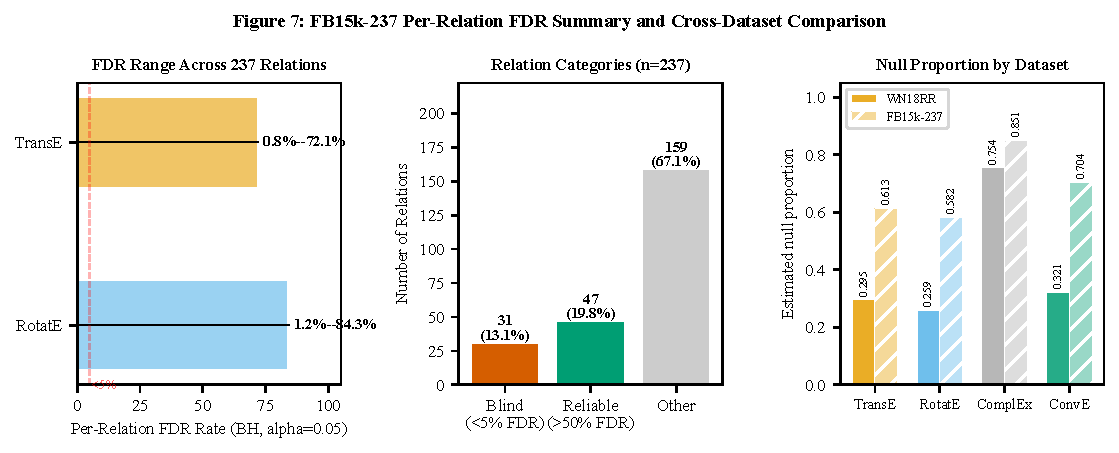
\includegraphics[width=\textwidth]{figures/fb15k237_per_relation_summary.pdf}
\caption{Cross-dataset FDR comparison. Left: per-relation raw $p < 0.05$ rate range for TransE and RotatE across 237 FB15k-237 relations. Center: distribution of relations into knowledge-blind ($<$5\% $p < 0.05$) and reliable ($>$50\% $p < 0.05$) categories. Right: estimated null proportion $\hat{\pi}_0$ for all four models on WN18RR (solid) versus FB15k-237 (hatched). $\hat{\pi}_0$ is consistently higher on the larger benchmark, and RotatE maintains the lowest $\hat{\pi}_0$ on both datasets.}
\label{fig:fb-cross}
\end{figure}

\subsection{Discussion}
\label{subsec:discussion}

\textbf{FDR framework as a diagnostic instrument.}
The experiments indicate that the proposed FDR framework can operate as a diagnostic instrument for KG embedding models, rather than merely offering an alternative evaluation metric.
It identifies:
\begin{itemize}
    \item The fraction of test triples for which the model carries no predictive signal ($\hat{\pi}_0$).
    \item Which relations the model handles reliably and which remain at chance level (relation-stratified FDR).
    \item Whether a higher MRR corresponds to a meaningful increase in statistically reliable discoveries (cross-model FDR comparison).
\end{itemize}

\textbf{Ablation of FDR components.}
To assess the incremental contribution of each FDR component, we compare three diagnostic layers independently: BH FDR control alone (binary discovery decisions at $\alpha = 0.05$), Storey's $q$-value estimation with $\hat{\pi}_0$ (which enables ranking hypotheses by FDR significance), and Efron's local FDR (which provides per-triple posterior null probabilities). Table~\ref{tab:fdr-overall} shows that these components yield complementary information: BH provides conservative but guaranteed error control, the $q$-value framework leverages $\hat{\pi}_0$ estimation to increase discovery power (e.g., TransE: $9.0\%$ BH vs.\ $63.0\%$ $q$-value, RotatE: $37.6\%$ BH vs.\ $70.1\%$ $q$-value), and the local FDR adds per-triple calibration that neither BH nor $q$-values supply. Notably, for ComplEx, all three methods agree: BH and $q$-value both report zero discoveries, and only 20 triples ($0.7\%$) pass the local FDR threshold---consistent with the model's $\hat{\pi}_0 = 0.754$ and near-random K-based MRR of $0.074$. The three components together form a coherent evaluation stack: BH for reliable discovery counting, $q$-values for fine-grained ranking, and local FDR for individual prediction calibration.

\textbf{Limitations and future work.}
We discuss five limitations.
First, the empirical $p$-value construction uses uniform negative sampling; more carefully designed null distributions, such as those obtained from type-constrained negative sampling~\cite{krompass2015type}, may yield better-calibrated $p$-values.
Second, while the present study provides results on WN18RR and FB15k-237 for four models, extending the analysis to larger datasets (e.g., YAGO3-10, CoDEx) and additional model families---particularly graph neural network-based encoders (CompGCN, NBFNet), hyperbolic embedders, and recent LLM-enhanced KG models---would further test the generality and scalability of the findings.
Third, the FDR framework treats negative samples as exchangeable; violations of this assumption---for instance, due to entity type constraints---could affect $p$-value validity and call for further study.
Fourth, the current results are reported from single training runs. KG embedding models exhibit predictive multiplicity~\cite{zhu2024predictive}, and FDR metrics may exhibit variance across random initializations. A supplementary multi-seed analysis across three model families---TransE, RotatE, and ConvE---under three random seeds each ($\{42, 123, 456\}$, 20 epochs, $K=100$) confirms that $\hat{\pi}_0$ and BH rejection rates are highly stable across initializations. Across all three models, the coefficient of variation (COV) for BH rejection rate is below $2\%$, and COV for $\hat{\pi}_0$ is below $6\%$ (TransE: $\hat{\pi}_0 = 0.287 \pm 0.004$, BH-R $= 29.4\% \pm 0.3\%$; RotatE: $\hat{\pi}_0 = 0.252 \pm 0.013$, BH-R $= 37.6\% \pm 0.5\%$; ConvE: $\hat{\pi}_0 = 0.320 \pm 0.001$, BH-R $= 25.3\% \pm 0.4\%$). Notably, RotatE's 20-epoch FDR metrics closely match its 100-epoch main-experiment results ($\hat{\pi}_0 = 0.259$, BH-R $= 37.6\%$), further supporting the stability of FDR-based model characterization. This tri-model evidence indicates that single-seed FDR comparisons are reliable, and the observed cross-model differences---particularly the $2.8\times$ ConvE--TransE BH rejection ratio---are driven by model architecture rather than random initialization. Extending multi-seed evaluation to ComplEx and to FB15k-237 would further strengthen these conclusions.
Fifth, the current evaluation does not include a real-world deployment case study.
While benchmark results establish the framework's statistical properties, evaluating its utility within a concrete knowledge-based application---such as clinical decision support, drug repurposing, or financial risk monitoring---would strengthen the argument that FDR-based reliability assessment translates to practical impact.
We consider all five directions important for follow-up work.
